\chapter{Antecedentes} \label{cap:antecedentes}

\section{Motor Rotativo de Combustión a Volumen Constante}
%
El MRCVC es un proyecto que surgió en la Universidad Nacional del
Comahue, inventado y patentado en el año 2004 por Jorge Toth\cite{toth}.
%
Actualmente se encuetra en desarrollo en el Departamento de Mecánica Aplicada
de la UNCo, en el marco del Proyecto de Investigación Desarrollo de modelos y
herramientas para la simulación de problemas complejos en ingeniería mediante
fluidodinámica computacional (04/I-251).

En trabajos anteriores\cite{lopez16, lopez13, roldan} se han mencionado las
características que hacen al MRCVC un motor atractivo. La geometría de la cámara
de combustión y del conjunto rotante permiten  combustión a volumen constante y
un balanceo mecánico de fuerzas.
%
Esto permite un funcionamiento más suave del motor, además de una reducción del
ruido y desgaste en comparación a motores rotativos tradicionales (Wankel) y
alternativos.


No obstante a esto hay que mencionar que los motores rotativos traen consigo una
serie de problemas como la necesidad de introducir aceite a la cámara de
combustión para lubricar elementos móviles, el solape de cámaras durante la
apertura de los puertos y en particular al MRCVC un complejo sistema de
sellos\cite{roldan}.



\section{Sistema de Intercambio de Gases}
%
Este sistema cumple la función de extraer los gases quemados de la cámara de
combustión de manera eficiente al final de cada carrera de expansión y de
admitir una carga de mezcla fresca para el próximo ciclo.
%
% En un motor de cuatro tiempos, el sistema suele estar compuesto por un filtro
% de aire,  tubo que conecta el filtro con el cuerpo de mariposa, cuerpo de
% mariposa, plenum de admisión y un puerto de admisión, como se ve en la
% figura \ref{fig:sist_intercambio}.
%
La masa de aire inductada imita la cantidad de combustible que se puede quemar,
por este motivo es importante tener un sistema de admisión eficiente.
%
De la misma manera, la cantidad de gases quemados que se pueden extraer luego de
cada ciclo limita la cantidad de masa fresca que puede ingresar a la cámara de
combustión.
%
Otros objetivos del sistema de intercambio de gases son el de preparar la
mezcla\footnote{En el caso de motores SI que admiten mezclas de aire y
combustible} y brindar un flujo que favorezca el proceso de combustión.

% \begin{figure}[h!] \centering
% 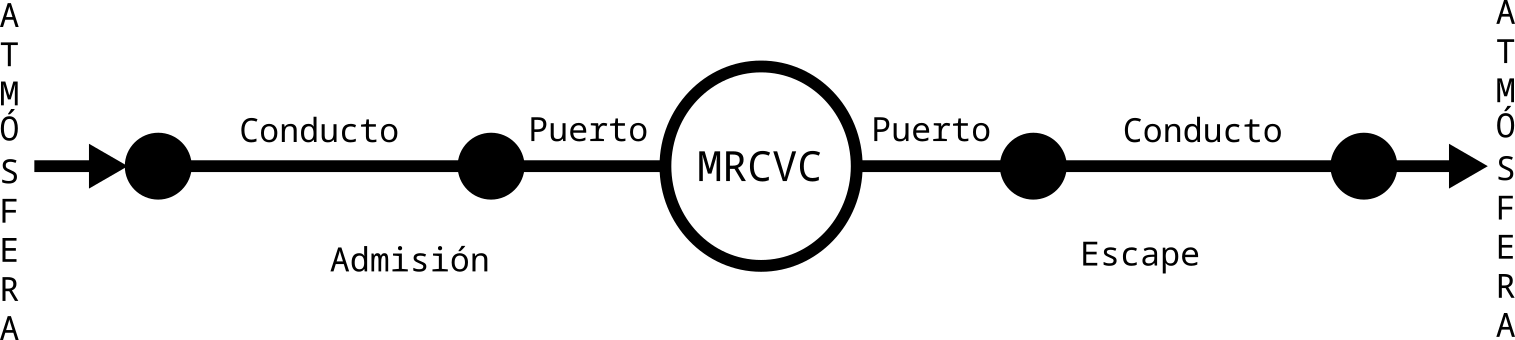
\includegraphics[width=0.5\textwidth]{sistema_intercambio_gases.png}
% \caption{Sistema de intercambio de gases esquematizado(buscar una libre o hacer
% un esquema propio)} \label{fig:sist_intercambio} \end{figure}

Para la simulación del MRCVC se usa una sistema simplificado, que consta de un
tubo de diámetro $D$ y longitud $L$ tanto para la admisión como para el escape,
como se ilustra en la figura \ref{fig:sist_int_mrcvc}.
%
La apertura y cierre de los puertos es controlada por la posición angular de los
puertos en el estator.

% \subsection{Solape de cámaras}
% %
% Es un proceso que ocurre en ambos puertos y que debe ser tenido en cuenta a la
% hora de evaluar el comportamiento del sistema de admisión y escape.
% %

\subsection{Indicadores de rendimiento}
\label{sec:indicadores_rendimiento}

Se medirá la eficiencia del sistema de intercambio de gases utilizando
exclusivamente el rendimiento volumétrico, $\eta_v$.
% Los conductos de admisión restringen el flujo de aire hacia el motor, para
% medir la eficiencia con la que se está admitiendo aire al motor se define el
% rendimiento volumétrico $\eta_v$.
%
Este se define como la relación entre el caudal volumétrico de aire que ingresa
al sistema de admisión y la velocidad a la que cambia el volumen dentro de un
cilindro.


\begin{equation}
  \label{eq:rendVol}
  \eta_v = \frac{2 \dot{m}_a}{\rho_{a,i} V_d N}
\end{equation}

Donde: $\rho_{a,i}$ es la densidad del aire a la entrada del sistema de
admisión (para motores naturalmente aspirados). También se puede definir
$\eta_v$ como:

\begin{equation}
    \label{eq:rendVol2}
    \eta_v = \frac{m_a}{\rho_{a,i} V_d}
\end{equation}

Dónde $m_a$ es la masa inductada al cilindro en cada ciclo.

Hay varios factores que afectan al rendimiento volumétrico, entre los más
importantes están:
%
\begin{enumerate}
    %
    \item Efectos cuasiestáticos
    %
    \item Pérdidas de carga por fricción viscosa
    %
    \item Pérdidas de carga en los puertos de admisión y escape
    %
    \item Transferencia de calor en sistema de admisión
    %
    \item Reglaje de los válvulas/puertos
    %
    \item Bloqueos de flujo en puertos de admisión y escape
    %
    \item Transferencia de calor en el cilindro
    %
    \item Sintonía del puerto de admisión y escape
    %
    \item Métodos de sobrecarga 
\end{enumerate}

Para este trabajo es de interés particular la pérdida de carga en los puertos,
el reglaje y la sintonía de admisión y escape.
%
En \cite{lopez13} se demostró que se tiene una mejor \emph{performance} del
motor si se ubican los puertos en el cuerpo central del estator, realizando un
optimización de la geometría mediante un barrido paramétrico de las variables
geométricas que determinan la forma, posición y reglaje de los puertos.
%
% La ubicación angular de los puertos determina la duración de los procesos de
% admisión y escape, además de modificar la forma y el coeficiente de descarga.

Estos parámetros se ajustan o seleccionan teniendo en cuenta requisitos de
funcionamiento del motor, por lo que fue necesario establecer una curva de
rendimiento volumétrico para que la simulación numérica del
ciclo termodinámico se pueda acoplar al algoritmo de optimización y de este
modo evaluar los motores contra la curva de rendimiento requerida.
%
El criterio de diseño/selección de la curva de $\eta_v$ fué el siguiente:

\begin{itemize}
  \item que tenga un pico de rendimiento entre 4000 y 6000 rpm.
  \item que la curva sea suave
\end{itemize}

% \subsubsection{Fracción de gases residuales}
% %
% A diferencia de un motor alternativo convencional en el que, por medio de
% métodos de sobrecarga se podría reducir la cantidad de gases residuales a una
% fracción despreciable, en el MRCVC, dada la disposición de la geometría siempre
% se transfiere gas residual desde una cámara que está transcurriendo por el
% barrido a la cámara contigua que está iniciando el proceso de admisión.

% Esta masa residual se puede calcular y depende del volumen atrapado y la preisón
% cuando cierra el puerto de escape.
% %
% Esta masa residual marca una cota inferior a la fracción de gases residuales
% que se pueden obtener, se menciona esto porque es un indicador del rendimiento
% de los sistemas de intercabmio de gases.
% %
% Considerando un motor con geometría perfecta y sin pérdida de masa entre los
% sellos, $x_{r\ min}$ se puede calcular como:

% $$
% x_{r\ min} = 0
% $$

% Considerando los valores gemoétricos utilizados para realizar esta optimización,
% este valor de $x_{r\ min}=0.1$ representa un objetivo para este trabajo.

% \subsection{Flujo a través de las válvulas}
% %
% Durante el escape, el soplido es un proceso que puede favorecer a la descarga
% de una cámara.

\subsection{Estrategias de simulación de motores}
%
Se simulará el motor con el simulador de motores de combustión interna ICEsym,
este simulador utiliza modelos 0D para la combustión y 1D para el flujo de
gases a través de los conductos (fuera de la cámara de combustión).

Esta es una herramienta muy útil ya que permite evaluar la \emph{performance} de
un motor a un costo computacional bajo además, la manera en que se implementó la
entrada y salida de datos permite utilizar este simulador como una ``caja
negra'' de modo que se pudo implementar en un \emph{script} como una función a
la que se le otorga como entrada un conjunto de parámetros y devuelve los
resultados de la simulación en un formato que permite la lectura y evaluación de
los mismos.
%
Esta característica del programa la que permitió acoplarlo con un algoritmo
genético para realizar la optimización de la geometría.


Como se mencionó en el apartado \ref{sec:indicadores_rendimiento}, en trabajos
previos se realizó un pre diseño de los puertos de admisión y escape.
%
En dicho trabajo se determinó coeficientes de descarga constantes
% En dicho trabajo se utilizaron coeficientes de descarga estimados y constantes
para simular el flujo en los puertos de admisión y escape.
%
Con el objetivo de modelar con mayor precisión el flujo a través de los puertos
se realizó una modificación al código de ICESym que permite utilizar una
variable adicional para modelar al $C_D$, con lo que se puede representar la
dependencia con la apertura del puerto como con la diferencia de presión
instantánea como $C_D = f(lv, \delta P)$.
